\documentclass[8pt,a4paper,compress]{beamer}

\usepackage{/home/siyer/lib/slides}

\title{Building a Computer}
\date{}

\begin{document}
\begin{frame}
\vfill
\titlepage
\end{frame}

\begin{frame}
\frametitle{Outline}
\tableofcontents
\end{frame}

\section{Numbers}
\begin{frame}[fragile]
\pause

At the most fundamental level, a computer manipulates electricity according to specific rules

\pause
\bigskip

To make those rules produce something useful, we need to associate the electrical signals with the numbers and symbols that we, as humans, like to use

\pause
\bigskip

To represent integers, computers use combinations of numbers that are powers of 2, called the base 2 or binary representation

\pause
\bigskip

With four consecutive powers $2^0, 2^1, 2^2, 2^3$, we can make all of the integers from 0 to 15 using 0 or 1 of each of the four powers

\pause
\bigskip

For example, $13 = 1 \cdot 2^3 + 1 \cdot 2^2 + 0 \cdot 2^1 + 1 \cdot 2^0 = 1101$; in other words, 1101 in base 2 means $1101 = 1 \cdot 2^3 + 1 \cdot 2^2 + 0 \cdot 2^1 + 1 \cdot 2^0$

\pause
\bigskip

This idea extends to other bases as well; For example, 603 in base 10 means $603 = 6 \cdot 10^2 + 0 \cdot 10^1 + 3 \cdot 10^0$ and 207 in base 8 means $207 = 2 \cdot 8^2 + 0 \cdot 8^1 + 7 \cdot 8^0$

\pause
\bigskip

In general, if we choose some base $b \geq 2$, every positive integer between 0 and $b^d-1$ can be uniquely represented using $d$ digits, with coefficients having values 0 through $b-1$

\pause
\bigskip

A modern 64-bit computer can represent integers up to $2^{64} - 1$
\end{frame}

\begin{frame}[fragile]
\pause

Arithmetic in any base is analogous to arithmetic in base 10

\pause
\bigskip

Examples of addition in base 10 and base 2
\begin{center}
\begin{tabular}{ccc}
  & 1 &   \\ 
  & 1 & 7 \\
+ & 2 & 5 \\
\hline
  & 4 & 2 \\
\end{tabular}\hspace{2cm} \begin{tabular}{ccccc}
  & 1 & 1 &   \\ 
  &   & 1 & 1 & 1 \\
+ &   & 1 & 1 & 0 \\
\hline
  & 1 & 1 & 0 & 1 \\
\end{tabular}
\end{center}

\pause
\bigskip

To represent a negative integer, a computer typically uses a system called two's complement, which involves flipping the bits of the positive number and then adding 1

\pause
\bigskip

For example, on an 8-bit computer, $3 = 00000011$, so $-3 = 11111101$
\end{frame}

\begin{frame}[fragile]
\pause

If we are using base 10 and only have eight digits to represent our numbers, we might use the first six digits for the fractional part of a number and last two for the exponent  

\pause
\bigskip

For example, 12345678 would represent $0.123456 \times 10^{78}$

\pause
\bigskip

Computers use a similar idea to represent fractional numbers, except that base 2 is used instead of base 10
\end{frame}

\section{Letters and Strings}
\begin{frame}[fragile]
\pause

In order to represent letters numerically, we need a convention on the encoding

\pause
\bigskip

The American National Standards Institute (ANSI) has established such a convention, called ASCII (American Standard Code for Information Interchange)

\pause
\bigskip

ASCII defines encodings for the upper- and lower-case letters, numbers, and a select set of special characters

\pause
\bigskip

ASCII, being an 8-bit code, can only represent 256 different symbols, and doesn't provide for characters used in many languages

\pause
\bigskip

The International Standards Organization's (ISO) 16-bit Unicode system can represent every character in every known language, with room for more

\pause
\bigskip

Unicode being somewhat wasteful of space for English documents, ISO also defined several ``Unicode Transformation Formats'' (UTF), the most popular being UTF-8 
\end{frame}

\begin{frame}[fragile]
\pause

A string is represented as a sequence of numbers, with a ``length field'' at the very beginning that specifies the length of the string

\pause
\bigskip

For example, in ASCII the sequence 99, 104, 111, 99, 111, 108, 97, 116, 101 translates to the string ``chocolate'', with the length field set to 9
\end{frame}

\section{Structured Information}
\begin{frame}[fragile]
\pause

We can represent any information as a sequence of numbers

\pause
\bigskip

Examples
\begin{itemize}
\item A picture can be represented as a sequence of pixels, each represented as three numbers giving the amount of red, green, and blue at that pixel

\item A sound can be represented as a temporal sequence of ``sound pressure levels'' in the air

\item A movie can be represented as a temporal sequence of individual pictures, usually 24 or 30 per second, along with a matching sound sequence
\end{itemize}
\end{frame}

\section{Boolean Algebra and Functions}
\begin{frame}[fragile]
\pause

Boolean variables are variables that take the value \lstinline{True} (1) or \lstinline{False} (0)

\pause
\bigskip

With booleans 1 and 0 we could use the operations (functions) \lstinline{AND}, \lstinline{OR}, and \lstinline{NOT} to build up more interesting boolean functions

\pause
\bigskip

A truth table for a boolean function is a listing of all possible combinations of values of the input variables, together with the result produced by the function

\pause
\bigskip

Truth tables for \lstinline{AND}, \lstinline{OR}, and \lstinline{NOT} functions

\begin{center}
\begin{tabular}{cc|c}
$x$ & $y$ & $x$ \lstinline$AND$ $y$ \\ \hline
0 & 0 & 0 \\
0 & 1 & 0 \\
1 & 0 & 0 \\
1 & 1 & 1
\end{tabular}\hspace{1cm} \begin{tabular}{cc|c}
$x$ & $y$ & $x$ \lstinline$OR$ $y$ \\ \hline
0 & 0 & 0 \\
0 & 1 & 1 \\
1 & 0 & 1 \\
1 & 1 & 1
\end{tabular}\hspace{1cm} \begin{tabular}{c|c}
$x$ & \lstinline$NOT$ $x$ \\ \hline
0 & 1 \\
1 & 0
\end{tabular}
\end{center}
\end{frame}

\begin{frame}[fragile]
\pause

Any function of boolean variables, no matter how complex, can be expressed in terms of \lstinline{AND}, \lstinline{OR}, and \lstinline{NOT}

\pause
\bigskip

For example, the ``implication'' function ($x \implies y$) described by the truth table
\begin{center}
\begin{tabular}{cc|c}
$x$ & $y$ & $x \implies y$ \\ \hline
0 & 0 & 1 \\
0 & 1 & 1 \\
1 & 0 & 0 \\
1 & 1 & 1
\end{tabular}
\end{center}
can be expressed as \lstinline{NOT} $x$ \lstinline{OR} $x$ \lstinline{AND} $y$ (or $\bar{x}+xy$)

\pause
\bigskip

An example of the implication function is ``if you score over 93\% in this course, then you will receive an A''
\end{frame}

\begin{frame}[fragile]
\pause

The minterm expansion algorithm, due to Claude Shannon, provides a systematic approach for building boolean functions from truth tables

\pause
\bigskip

Minterm expansion algorithm
\begin{enumerate}
\item Write down the truth table for the boolean function under consideration

\item Delete all rows from the truth table where the value of the function is 0

\item For each remaining row, create something called a ``minterm'' as follows
\begin{enumerate}[a.]
\item For each variable that has a 1 in that row, write the name of the variable. If the input variable is 0 in that row, write the variable with a negation symbol to \lstinline{NOT} it

\item Now \lstinline{AND} all of these variables together
\end{enumerate}

\item Combine all of the minterms for the rows using \lstinline{OR}
\end{enumerate}

\pause
\bigskip

For the implication function, the minterm expansion algorithm produces the boolean function $\bar{x}\bar{y}+\bar{x}y+xy$, which is equivalent to the simpler $\bar{x}+xy$ function

\pause
\bigskip

Finding the simplest form of a boolean function is provably as hard as some of the hardest (unsolved) problems in mathematics and computer science
\end{frame}

\section{Logic Using Electrical Circuits}
\begin{frame}[fragile]
\pause

An electromechanical switch in which when the input power is off, the output is ``low'' (0), and when the input power is on, the output is ``high'' (1)
\begin{center}
\visible<2->{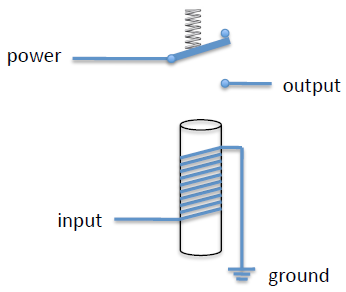
\includegraphics[scale=0.22]{figures/em_switch.png}}
\end{center}

\pause
\bigskip

Devices (\lstinline{AND} and \lstinline{OR} gates) for computing $x$ \lstinline{AND} $y$ and $x$ \lstinline{OR} $y$, constructed using electromechanical switches
\begin{center}
\visible<3->{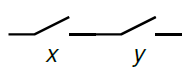
\includegraphics[scale=0.22]{figures/and_gate.png}\hspace{1cm} 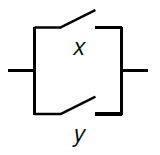
\includegraphics[scale=0.22]{figures/or_gate.png}}
\end{center}

\pause
\bigskip

The function \lstinline{NOT} $x$ can be implemented by constructing a switch that conducts if and only $x$ is 0
\end{frame}

\begin{frame}[fragile]
\pause

Computers today are built with much smaller, much faster, more reliable, and more efficient transistorized switches 

\pause
\bigskip

Since the details of the switches aren't terribly important at this level of abstraction, we represent, or ``abstract'', the gates using the following symbols
\begin{center}
\visible<3->{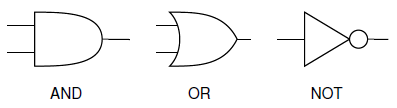
\includegraphics[scale=0.3]{figures/gate_symbols.png}}
\end{center}

\pause
\bigskip

A logical circuit for the implication function $\bar{x}\bar{y}+\bar{x}y+xy$
\begin{center}
\visible<4->{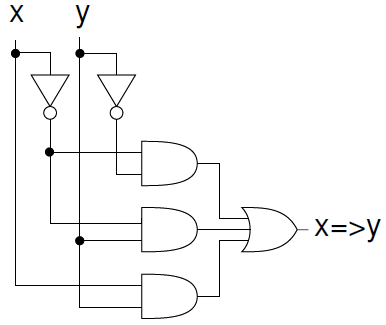
\includegraphics[scale=0.22]{figures/implication_circuit.png}}
\end{center}
\end{frame}

\section{Computing With Logic}
\begin{frame}[fragile]
\pause

A truth table describing the addition of two two-bit numbers to get a three-bit result
\begin{center}
\begin{tabular}{cc|c}
$x$ & $y$ & $x +y$ \\ \hline
00 & 00 & 000 \\
00 & 01 & 001 \\
00 & 10 & 010 \\
$\vdots$ & $\vdots$ & $\vdots$ \\
01 & 10 & 011 \\
01 & 11 & 100 \\
$\vdots$ & $\vdots$ & $\vdots$ \\
11 & 11 & 110
\end{tabular}
\end{center}

\pause
\bigskip

Building a corresponding circuit using the minterm expansion algorithm is infeasible --- adding two 16-bit numbers, for example, will result in a circuit with several billion gates
\end{frame}

\begin{frame}[fragile]
\pause

We build a relatively simple circuit called a full adder (FA) that does just one column of addition

\pause
\bigskip

We can ``chain'' $n$ full adders together to add two $n$-bit numbers;  The resulting circuit is called a ripple-carry adder

\pause
\bigskip

A 2-bit ripple-carry adder
\begin{center}
\visible<4->{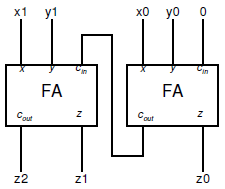
\includegraphics[scale=0.4]{figures/ripple_carry_adder.png}}
\end{center}
\end{frame}

\section{Memory}
\begin{frame}[fragile]
\pause

Truth table for a \lstinline{NOR} gate (\lstinline{OR} followed by \lstinline{NOT})
\begin{center}
\begin{tabular}{cc|c}
$x$ & $y$ & $x$ \lstinline$NOR$ $y$ \\ \hline
0 & 0 & 1 \\
0 & 1 & 0 \\
1 & 0 & 0 \\
1 & 1 & 0
\end{tabular}
\end{center}

\pause
\bigskip

A latch is a device that allows us to ``lock'' a bit and retrieve it later

\pause
\bigskip

By aggregating millions of latches we have the Random Access Memory (RAM)

\pause
\bigskip

A latch can be constructed from two \lstinline{NOR} gates as shown below
\begin{center}
\visible<5->{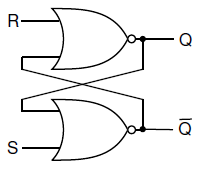
\includegraphics[scale=0.4]{figures/latch.png}}
\end{center}
where the input $S$ is known as ``set'' while the input $R$ is known as ``reset''
\end{frame}

\section{von Neumann Architecture}
\begin{frame}[fragile]
\pause

In a modern computer, the CPU (Central Processing Unit) is where all the computation takes place

\pause
\bigskip

The CPU has devices such as ripple-carry adders, multipliers, etc. for doing arithmetic. In addition, it has a small amount of (scratch) memory called registers

\pause
\bigskip

The computer's main memory, which allows storing large amounts of data, is separate from the CPU and is connected to it by wires on the computer's circuit board

\pause
\bigskip

A program, which is usually a long list of instructions, is stored in the main memory, and is copied, one instruction at a time, into a register in the CPU for execution

\pause
\bigskip

The CPU has two special registers: a program counter that keeps track of the location in memory where it will find the next instruction and an instruction register that stores the next instruction to execute

\pause
\bigskip

This way of organizing computation is due to the famous mathematician and physicist, John von Neumann, and is known as the von Neumann architecture
\end{frame}

\begin{frame}[fragile]
\pause

Instructions, like data, can be encoded as numbers

\pause
\bigskip

For example, let's assume an 8-bit computer with only four instructions: add, subtract, multiply, and divide

\pause
\bigskip

Each of the instructions will need a number, called an operation code (or opcode), to represent it
\begin{center}
\begin{tabular}{cc}
Opcode & Meaning \\ \hline
00 & Add \\
01 & Subtract \\ 
10 & Multiply \\
11 & Divide
\end{tabular}
\end{center}

\pause
\bigskip

Next, let's assume that our computer has four registers, numbered 0 through 3, and 256 8-bit memory cells

\pause
\bigskip

An instruction will be encoded as: the first two bits represent the instruction, the next two bits encode the ``destination register'', the next four bits encode the registers containing two operands

\pause
\bigskip

For example, the instruction \lstinline{add 3 0 2} (meaning add the contents of register 2 with the contents of register 0 and store the result in register 3) will be encoded as \lstinline{00110010}
\end{frame}

\begin{frame}[fragile]
\pause

Our computer operates by repeatedly performing the following procedure
\begin{enumerate}
\item Send the address in the program counter (commonly called the PC) to the memory, asking it to read that location

\item Load the value from memory into the instruction register

\item Decode the instruction register to determine what instruction to execute and which registers to use

\item Execute the requested instruction, which involves reading operands from registers, performing arithmetic, and sending the results back to the destination register

\item Increment PC so that it contains the address of the next instruction in memory
\end{enumerate}

\begin{center}
\visible<2->{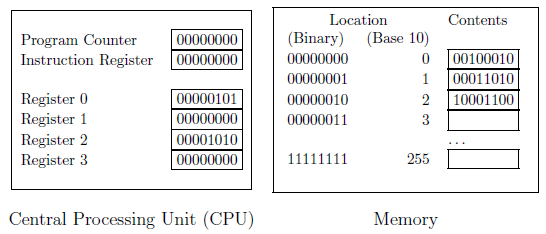
\includegraphics[scale=0.35]{figures/von_neumann_arch.png}}
\end{center}
\end{frame}
\end{document}
